%----------------------------------------------------------------------------------------
%	LEFT COLUMN
%----------------------------------------------------------------------------------------

\begin{minipage}[t]{0.33\textwidth} % The left column takes up 33% of the text width of the page


\section{Education} 
\runsubsection{PhD}
\descript{| Electrical and Computer Engineering}
\location{University of Oklahoma (OU) | 2018-Present}
\vspace{\topsep} % Hacky fix for awkward extra vertical space
\vspace{1pt}
\begin{tightitemize}
\item Research: Augmented Surgical Reality, Computer Vision, Deep Learning
\item Honor: Graduate Fellowship
\item GPA: 4
\item Advisor: \href{http://www.ou.edu/coe/ece/faculty_directory/dr_cheng}{Dr. Samuel Cheng} 
\end{tightitemize}
\vspace{6pt}

\runsubsection{BS}
\descript{| Electrical and Electronic Engineering}
\location{United International University (UIU), Bangladesh | 2014}
\begin{tightitemize}
\item Concentration in wireless communications
\item Honors: Graduated Magna Cum Laude, Top 2 \% class standing, Full tuition \& fees waiver scholarships
\item GPA: 3.93
\end{tightitemize}


\sectionspace % Some whitespace after the section
%------------------------------------------------
% Coursework
%------------------------------------------------

\section{Graduate Coursework}
Machine Learning for Engineers \\
Advanced Artificial Neural Networks \\
Artificial Neural Networks \& Applications
Numerical Analysis \\

%------------------------------------------------
% Skills
%------------------------------------------------
\sectionspace % Some whitespace after the section

\section{Skills}

\descript{Languages}
\location{Experienced}
\textbullet{} Python (2 years) \textbullet{}  Matlab (5 years) \\ 
\location{Proficient}
\textbullet{} R \textbullet{} C++ \textbullet{} C \\
\sectionspace % Some whitespace after the section

\descript{Machine Learning}
\location{Frameworks}
\textbullet{} PyTorch \textbullet{} Tensorflow \textbullet{} Pandas \\
\textbullet{} Scikit-Learn \textbullet{} Keras\\ 
\location{Algorithms}
\textbullet{} CNN \textbullet{} GAN \textbullet{} LSTM \textbullet{} RNN\\
\sectionspace % Some whitespace after the section

\descript{Game Engine and 3D Software}
\textbullet{} Unreal Engine 4 \textbullet{} Blender
\sectionspace % Some whitespace after the section

\descript{General}
\location{OS}
\textbullet{} Linux \textbullet{} Windows\\ 
\location{Web}
\textbullet{} HTML\textbullet{} CSS\textbullet{} jQuery\textbullet{} javaScript\textbullet{} PHP\textbullet{} CodeIgniter\textbullet{} MySql
\\

\end{minipage} % The end of the left column
\hfill
%
%----------------------------------------------------------------------------------------
%	RIGHT COLUMN
%----------------------------------------------------------------------------------------
%
\begin{minipage}[t]{0.66\textwidth} % The right column takes up 66% of the text width of the page

%------------------------------------------------
% Experience
%------------------------------------------------

\section{Experience}

\runsubsection{Image and Information Processing Lab, OU}\\
\descript{Graduate Research Assistant} 
\location{Aug 2018 - Present}
\vspace{\topsep} % Hacky fix for awkward extra vertical space
\begin{tightitemize}
\item Conducting research on Augmented Surgical Reality.
\item Applying PyTorch and Tensorflow for 6 DoF pose estimation of surgical tools.
\item Experimenting with the usability of depth-sensing cameras in operation room lighting. Cameras include Intel D435i, Stereolabs Zed, Microsoft Kinect-2 and MYNTEYE S1030.
\item Porting Python projects into C++ applications for Microsoft Hololens.
\item Creating 3D object models and salvaging 3D scanned models using Blender. 
\item Generating synthetic training-data using Unreal Engine 4 for deep-learning.

\end{tightitemize}

\sectionspace % Some whitespace after the section


%------------------------------------------------

\runsubsection{Biomedical, Image and Signals Research Group, UIU}\\
\descript{Research Assistant (Full-time)}
\location{Nov 2016 - July 2018  (1 year 9 months)}
\begin{tightitemize}
\item Conducted research on development of a low-cost technology for screening microvascular complications in diabetic population in Bangladesh.
\item Extensive usage of Matlab for data preprocessing, signal processing, machine learning and app development for live-capturing and cleaning medical signals.
\item Data acquisition and management: ECG and PPG, Cardiovascular Reflex Test, Fundus Photography, Nerve Conduction Velocity, and Blood Tests.
\item Project management: Equipment procurement \& modification, protocol development, collaboration with physicians, budget distribution, ethical approval acquisition, management of other RAs and thesis students.
\item Side Project: Detection of fECG R-R peak locations using machine learning.
\end{tightitemize}
\sectionspace % Some whitespace after the section

%------------------------------------------------

\runsubsection{National University of Malaysia}\\
\descript{Graduate Research Assistant}
\location{October 2015 - June 2016 (9 months)}
\begin{tightitemize}
\item Conducted research on the forward error correction block of ZigBee based baseband processor.
\end{tightitemize}
\sectionspace % Some whitespace after the section

%------------------------------------------------

\runsubsection{United International University, Bangladesh}\\
\descript{Research Assistant (Full-time)}
\location{February 2015 - June 2015 (5 months)}
Wireless Power Transfer, a Joint Research Collaboration with University of Saskatchewan, Canada.
\begin{tightitemize}
\item Developed Matlab based program for optimum wireless power transfer and tested validity in hardware.
\end{tightitemize}
\sectionspace % Some whitespace after the section

\descript{Teaching Assistant}
\location{October 2014 - January 2015 (4 months)}
\begin{tightitemize}
\item Digital Signal Processing and Electrical Circuits 1
\end{tightitemize}
\sectionspace % Some whitespace after the section

\descript{Research Assistant (Full-time)}
\location{April 2014 - September 2014 (6 months)}
Computer Vision-Based Wireless Capsule Endoscopy (WCE) Tracking, a joint Research Collaboration with University of Saskatchewan, Canada.
\begin{tightitemize}
\item Developed a computer vision system and a 3D virtual intestine in Matlab for localizing WCE PillCam inside human intestine.
\end{tightitemize}
\sectionspace % Some whitespace after the section
%------------------------------------------------

%----------------------------------------------------------------------
\tikz[remember picture,overlay] \node[xshift=-3.25cm, yshift=1.5cm, opacity=0.3] at (current page.south east){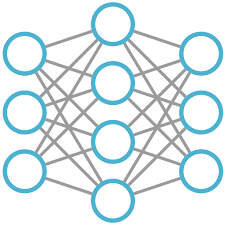
\includegraphics[width=0.8in,height=0.8in]{incon_neural_net.png}};

\end{minipage} % The end of the right column
\vspace*{\fill}
\center{\textcolor{gray}{1/2}}